\subsection{Funktionsnachweis kritischer Funktionen}
Dieses Unterkapitel befasst sich mit dem praktischen Nachweis von kritischen Teilfunktionen. Kritische Teilfunktionen sind Funktionen, welche bei einem Ausfall dieser Teilfunktion, einen Ausfall des Gesamtsystems zur Folge hat. Dabei soll die Umsetzung einfacher Funktionsmuster einen praktischen Nachweis bringen, sodass die Umsetzung von dieser Teillösung legitimiert ist.
\newline
Bei genauerer Betrachtung der Funktionsanalysen (Abbildungen \ref{fig:FunktPflicht} und \ref{fig:FunktWunsch}) ist erkennbar, dass beide Varianten (Pflicht sowie Wunsch) eine Serieschaltung darstellen. Bei einer Umsetzung einer Maschine mit einfacher Redundanz ergibt dies implizit, dass jede Funktion als kritisch eingestuft werden kann. Aus zeitlichen Gründen kann ein umfassenden Nachweis von allen Teillösungskonzepten nicht abschliessend durchgeführt werden. Eine pragmatische Auswahl von Funktionen mit erhöhtem Ausfallrisiko und einer vielversprechenden Funktionserfüllung wird daher angestrebt.

\subsubsection{NemaCaps vereinzeln}
\subsubsection{NemaCaps fördern}
\subsubsection{NemaCaps setzen}
Ein Lösungsansatz der Teilfunktion "NemaCaps setzen" basiert auf der Idee zuerst ein Loch auszuheben oder zu verdrängen und dann ein NemaCap ins Loch fallen zu lassen. Ähnlich ist eine andere Idee, welche mit einer spitzen Zange das Loch verdrängt wird, sich die Zange in der Erde öffnet und so ein NemaCap platziert.
\newline
Um die Umsetzbarkeit dieser Ideen zu überprüfen, werden zwei Versuche durchgeführt:
\begin{itemize}
	\item \textbf{A) Ermittlung der Verdrängkraft:} Mit einer konventionellen Setzhilfe aus dem Gartenbau werden praktische Tests durchgeführt. Dabei wird ein Topf mit dem vorgegebenen Gartenhumus von Ricoter befüllt und leicht angepresst. Nun wird die maximale Einsetztiefe an der Setzhilfe markiert und schrittweise mit Gewicht (Masse m in Abbildung \ref{fig:skizze_setzversuch}) beschwert. Sobald die Markierung den Gartenhumus berührt, wird die Setzhilfe inklusive Masse m gewogen und durch die Multiplikation mit der Erdbeschleunigung die benötigte Verdrängkraft ermittelt.
	
	\item \textbf{B) NemaCap mittels Zange setzen:} Der identische Versuch wird mit der genannten Zange durchgeführt. Zusätzlich wird in die geschlossene Zange ein NemaCap gegeben. Bei Erreichung der Setztiefe wird die Zange geöffnet und das NemaCap platziert. Realisiert wird die Zange aus gelasertem MDF.
\end{itemize} 

\begin{figure}[H]
	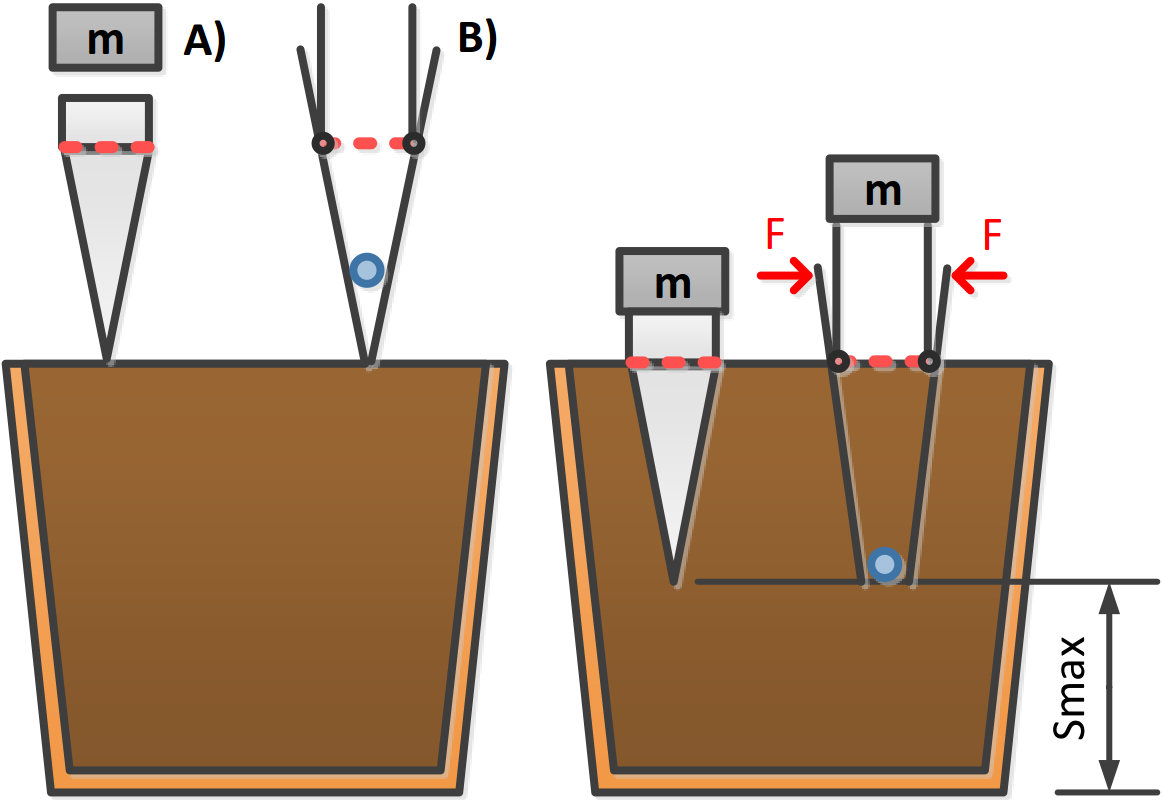
\includegraphics[width=1\textwidth]{Illustrationen/5-Konzept/skizze_stechversuch.PNG}
	\caption{Versuchsaufbau zur Ermittlung der Verdrängkraft}
	\label{fig:skizze_setzversuch}
\end{figure}

\textbf{Erkenntnisse}
\newline
Folgende Erkenntnisse lieferten die Versuche:
\begin{itemize}
	\item Mit der konventionellen Setzhilfe kann mit geringem Aufwand das erforderliche Setzloch verdrängt werden. Auch bei erschwerten Umständen wie komprimiertem Gartenhumus oder kleinerem Gehölz im Humus konnte ein Setzloch verdrängt werden. Über mehrere Versuche wurden folgende Werte ermittelt:
	\begin{tabular}{|l|c|c|}
		\hline 
		& kleinster Topf (D=90mm) & grösster Topf (D=140mm) \\ 
		\hline 
		geforderte Setztiefe [mm] & 40 & 64 \\ 
		\hline 
		benötigte Masse [kg] & 0.15 & 0.6 \\ 
		\hline 
		Verdrängungskraft[N] & 1.5  & 6.0  \\ 
		\hline 
	\end{tabular} 
	
	\item Der gegebene Gartenhumus von Ricoter besitzt gute Eigenschaften für diese Anwendung. Nach der Verdrängung behält das Setzloch seine Form bei, sodass die Bedingungen für das Einsetzen des NemaCaps gegeben sind. Dabei ist darauf zu achten, dass stets frischer Gratenhumus verwendet wird.
	
	\item Tests mit der Zange ergaben, dass eine Verdrängung der Erde mit dem identischen Kraftaufwand machbar ist. In der erforderlichen Setztiefe angekommen, benötigt es einen erhöhten Kraftaufwand, um die Zange zu öffnen und das NemaCap zu platzieren. Wie eine Streckenlast wirkt die zu verdrängende Erde der Bewegung entgegen und erschwert die Öffnung. Diese Teillösung wird als nicht umsetzbar eingeschätzt.
\end{itemize} 

\subsubsection{Setzmechanismus konfigurieren}







Basierend auf der funktionsbezogenen Variation der Aufgabenstellung werden in diesem Unterkapitel interessante Teillösungskonzepte genauer betrachtet.

Der Fokus liegt dabei auf Funktionen, welche als kritisch beurteilt werden.


 Gemeint sind dabei Funktionen, für welche keinen Nachweis existiert, dass ein Einsatz von NemaCaps zuverlässig funktioniert.

 Primär sollen Teillösungskonzepte betrachtet werden deren Funktionserfüllung vielversprechend ist, jedoch keinen praktischen Nachweis für diese Anwendung existiert oder noch nie mit NemaCaps angewandt wurde. . Gemeint sind Teillösungskonzepte